As mentioned in the previous introductory section, Proof-of-Work (PoW) is defined as the \textbf{consensus algorithm} of the entire Bitcoin network.\\\\
However, the term "Proof of Work" was born even before Bitcoin began, since it was introduced by the cryptographer Adam Back, in his work on the so-called \textbf{Hashcash} system: <<Hashcash was originally proposed as a mechanism to throttle systematic abuse of un-metered internet resources such as email, and anonymous remailers in May 1997.>> \cite{back2002hashcash} The basic idea behind Hashcash was to require a computational effort from the sender of a message, making it costly and time-consuming to send a large number of messages or launch coordinated attacks. In order to send an email to a Hashcash user, the sender would have to find a hash of the email that fell within a certain range. Since a hash is a large, unpredictable number, producing such a hash takes many guesses. Once the valid hash was found, the sender could include it in the message header. In this way, the recipient was able to immediately verify the validity of the result contained in the message header. In that case, the Proof-of-Work system was intended as a method to combat email spam and denial-of-service attacks. Satoshi Nakamoto, while designing the Bitcoin protocol, most likely took inspiration from it: for this reason Hashcash is also considered a precursor to the Bitcoin consensus algorithm.\\
Moreover, with his invention, the creator of Bitcoin was able to solve with a practical solution a very known problem in distributed computing, defined as the \textbf{Byzantine Generals' Problem}. This concept can be understood by reading the first lines of the original paper which described and gave birth to the term itself: <<Reliable computer systems must handle malfunctioning components that give conflicting information to different parts of the system. This situation can be expressed abstractly in terms of a group of generals of the Byzantine army camped with their troops around an enemy city. Communicating only by messenger, the generals must agree upon a common battle plan. However, one or more of them may be traitors who will try to confuse the others. The problem is to find an algorithm to ensure that the loyal generals will reach agreement.>> \cite{journals/toplas/LamportSP82}\\
Bitcoin found definitely a solution to this, by introducing the concept of Proof of Work as the foundational problem to solve during mining operations. In this way it also found a way to ensure that users could agree on a single state of the ledger, at the same time avoiding any \textbf{double spending} attempts or other invalid transactions. To summarize, PoW in Bitcoin definitely enabled consensus without relying on a central trusted authority.\\\\
The other innovative concept introduced in Bitcoin, is the above-mentioned mechanism called \textbf{difficulty adjustment}. It's a fundamental piece of the entire protocol, since it allows the network to automatically regulate the level of difficulty associated with mining a block. The difficulty adjustment is based on the mining speed of participants in the network. By dynamically adjusting the mining difficulty, increasing or decreasing the range of valid hash results, Bitcoin ensures that new coins are produced at a predetermined rate, one block every 10 minutes (on average), regardless of the total computing power dedicated to mining. This automatic adjustment mechanism is done every 2016 blocks mined (about 2 weeks), and it contributes to the network's resilience and scalability, preventing issues like hyperinflation or compromised security. From an economic perspective, the difficulty adjustment is a unique mechanism which provides a never discovered property for something who can aspire to be used as money. As perfectly stated by the economist Saifedean Ammous, in his great work "The Bitcoin Standard":
<<For anything to function as a good store of value, it has to beat this trap: it has to appreciate when people demand it as a store of value, but its producers have to be constrained from inflating the supply significantly enough to bring the price down.>>\cite{bitcoinstandard}\\
This is a very unique discovery, since every form of money before Bitcoin has always followed the following rule: the more the good used as money appreciated, because of a demand growth for it, the more it has been produced. In this case, very uniquely, the demand for the good used as money (bitcoin) will never be able to modify (by increasing or decreasing) the offer of it. This property guarantees that Bitcoin supply in almost perfectly inelastic, since the production rate on newly minted bitcoin is totally determined by the difficulty adjustment mechanism.
\begin{figure}[h!]
\centering
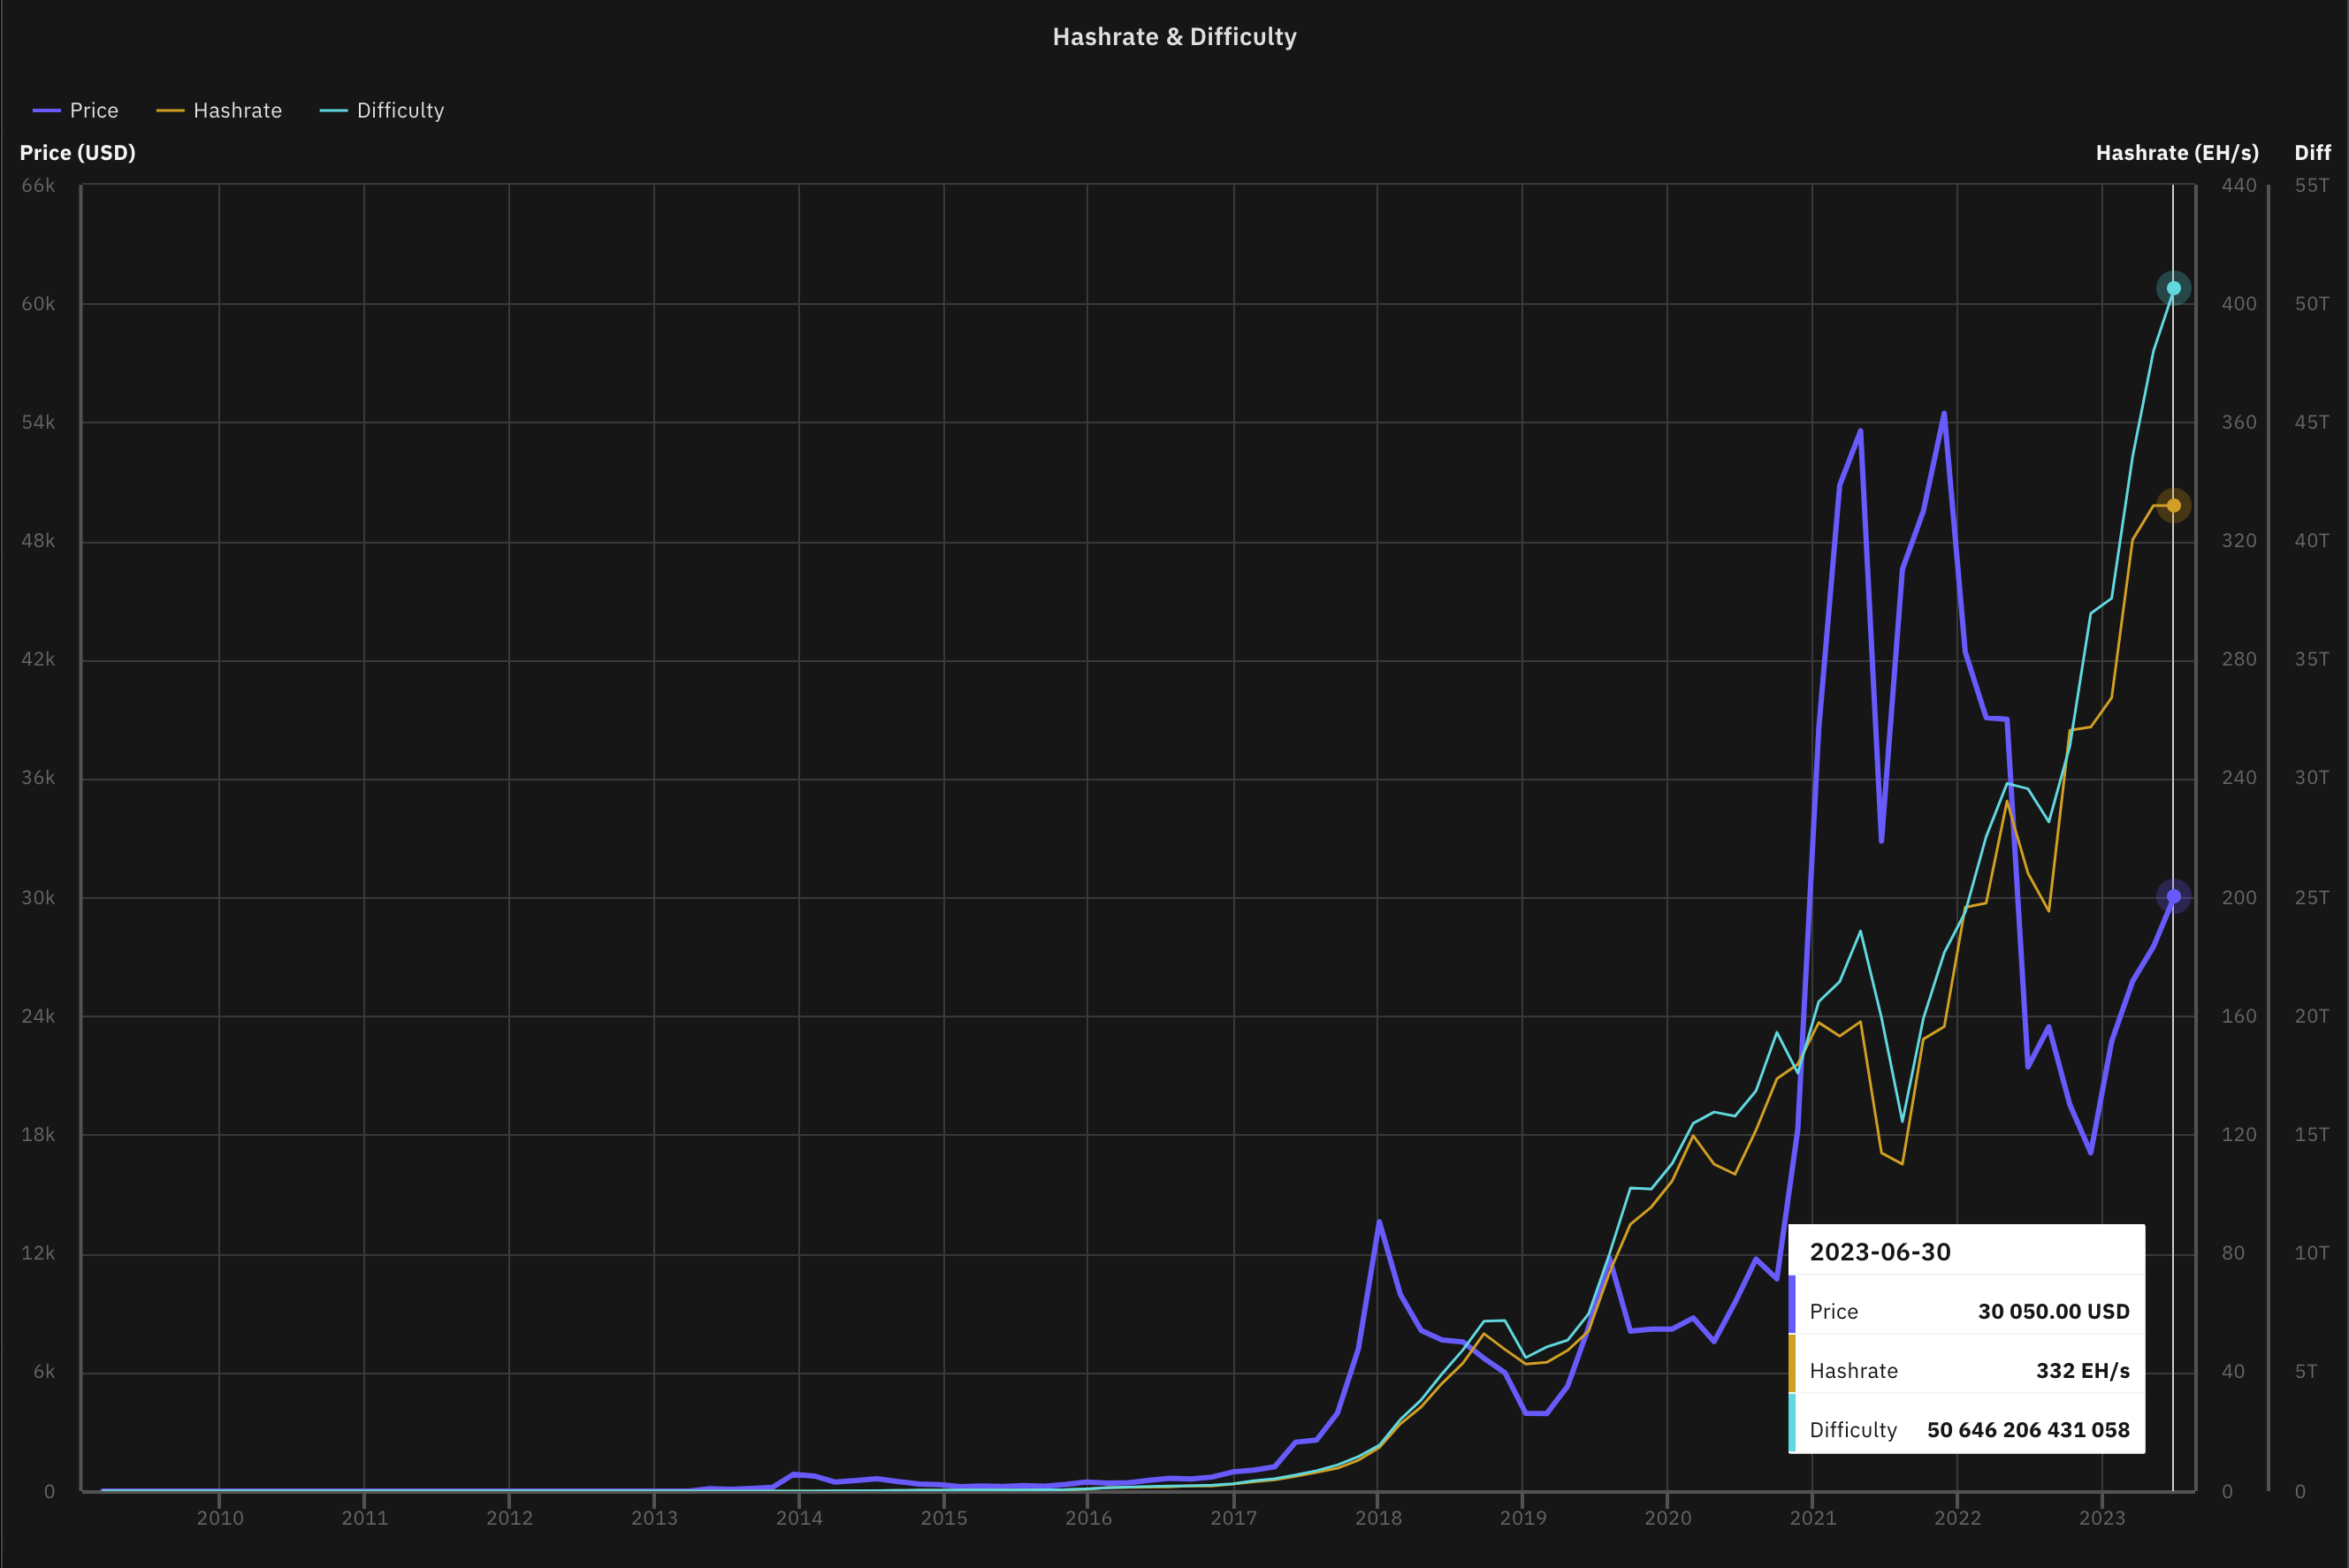
\includegraphics[width=14cm]{Figures/bitcoin/difficulty-2.png}
\caption{Price, hashrate and difficulty representation, \href{https://insights.braiins.com/en}{\textit{insights.braiins.com}}}
\label{fig:difficulty}
\end{figure}

\noindent Furthermore, Bitcoin introduced the notion of blockchain \textbf{immutability}, ensuring the integrity of past transactions. Each new block is added to the end of the existing blockchain, forming an unbreakable chain of transactions. Modifying a past transaction would require rewriting the entire block containing the transaction and all subsequent blocks. Additionally, the attacker would need to generate new blocks at a faster rate than the entire Bitcoin network combined in order to catch up and create a longer chain, which is practically infeasible.\\\\

\noindent In summary, the combination of PoW, difficulty adjustment, which regulates the rate of coin emission, and the immutability of the blockchain, which fortifies past transactions, contribute to the decentralized and secure nature of the Bitcoin network. These features allow Bitcoin to operate autonomously and efficiently without relying on a central authority.

